Um circuito comumente utilizado para a implementação do retificador monofásico de ponto médio alimentado por um transformador pode ser observado na figura \ref{fig:RMOCDPM}. 

\begin{figure}[ht]
\center
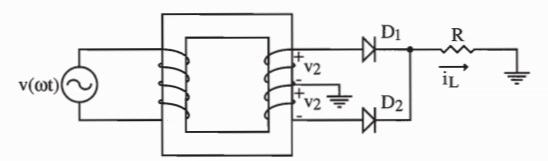
\includegraphics[scale=0.9]{imagens/ret_mono_ondaCompleta_cargaResistiva.PNG}
\caption{Retificador monofásico a diodo de onda completa com ponto médio, com carga puramente resistiva.}\label{fig:RMOCDPM}
\caption*{Fonte: Eletrônica de Potência (2006)}
\end{figure}

Pela análise desse circuito podemos notar que ele possui duas etapas de funcionamento relativas aos momentos de condução de cada um dos diodos. Ou seja, em cada semiciclo da fonte de alimentação, um dos diodos entra em condução. Como eles estão conectados de forma simétrica em relação ao ponto médio do enrolamento no secundário do transformador, a tensão aparente à carga em cada uma dessas etapas de funcionamento é idêntica. A figura \ref{fig:EFCR} demonstra essas etapas de funcionamento.

\begin{figure}[ht]
\center
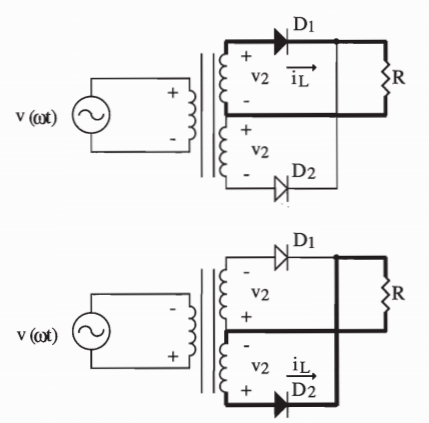
\includegraphics[scale=1.2]{imagens/etapas_funcio_ondaComp_pontoMedio.PNG}
\caption{Etapas de Funcionamento do circuito retificador de onda completa com ponto médio.}\label{fig:EFCR}
\caption*{Fonte: Eletrônica de Potência (2006)}
\end{figure}

O valor médio da tensão na carga pode ser modelado por
\begin{align*}
    V_{L,med} &= \frac{1}{\pi}{\int_{0}^{\pi}}{\sqrt{2}V_2{\sin(\omega{t})d(\omega{t})}} \\
	      &= 0,9 V_2 \\
    \implies I_{L,med} &= \frac{0,9 V_2}{R}
.\end{align*}

A corrente de pico na carga e nos diodos pode ser descrita por \[
I_{p} = \frac{\sqrt{2}V_2}{R}
.\] Dessa forma, a tensão de pico inversa dos diodos é \[
V_{Dp} = {2}\sqrt{2}V_2
.\] 

O valor médio da corrente em cada diodo é igual à metade do valor médio da corrente na carga, portanto \[
I_{D,med} = \frac{0,9 V_2}{2R}
.\] 

Os valor eficaz da corrente na carga é \[
I_{L,ef} = \frac{V_2}{R}
.\] 

Mesmo em um circuito em que a carga possui um componente indutivo, como na figura \ref{fig:ROCACI}, as etapas de funcionamento são as mesmas descritas para a carga resistiva pura.

\begin{figure}[ht]
\center
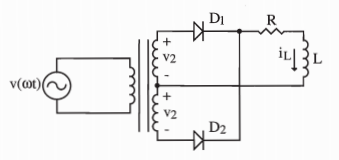
\includegraphics[scale=1.4]{imagens/CargaRL_ondaComple_pontoMedio.PNG}
\caption{Retificador de onda completa com ponto médio com uma carga com componente indutivo.}\label{fig:ROCACI}
\caption*{Fonte: Eletrônica de Potência (2006)}
\end{figure}

Para obter o equacionamento da corrente na carga novamente utiliza-se a série de Fourier, de forma que
\begin{align*}
    V_{L}(\omega{t}) &= \sqrt{2}V_2[{\frac{2}{\pi}-\frac{4}{3\pi}{\cos({2\omega}{t})}} - \frac{4}{15\pi}{\cos(4{\omega}{t})} - ...] \\
    I_{L}(\omega{t}) &= \sqrt{2}V_2[{\frac{2}{R\pi}-\frac{4}{3\pi{Z_2}}{\cos({2\omega}{t}-\phi_2)}} - \frac{4}{15\pi{Z_4}}{\cos(4{\omega}{t}-\phi_4)} - ...]
,\end{align*}
em que
\begin{align*}
Z_n &= \sqrt{R^2 + {n^2}{\omega}{L^2}} \text{, e} \\
\phi_n &= \tan^{-1}(\frac{n{\omega}{L}}{R})
.\end{align*}

Assim, obtém-se a corrente e tensão médias na carga modeladas por
\begin{align*}
    I_{L,med} &= \frac{2\sqrt{2}{V_2}}{\pi{R}} = \frac{0,9 V_2}{R} \\
    V_{L,med} &= 0,9 V_2
,\end{align*}
logo, \[
I_{D,med} = \frac{0,45 V_2}{R}
.\] 

O valor eficaz da corrente num diodo é \[
I_{D,ef} = 0,707{I_{L,med}}
.\] 

Dessa forma, vemos que a tensão e a corrente na carga segue como ilustrado na figura \ref{fig:TCCROCACI}.

\begin{figure}[ht]
\center
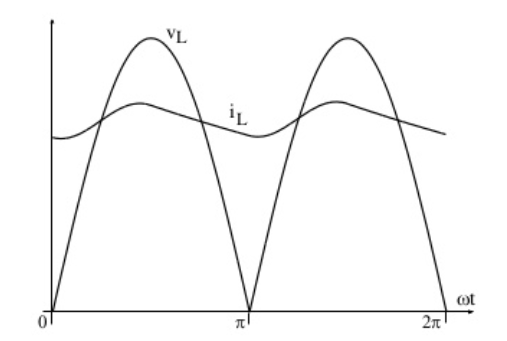
\includegraphics[scale=1.0]{imagens/tensaocorrentedecarga.PNG}
\caption{Tensão e corrente de carga para o circuito da figura \ref{fig:ROCACI}.}\label{fig:TCCROCACI}
\caption*{Fonte: Eletrônica de Potência (2006)}
\end{figure}

Para entender o comportamento da tensão e da corrente no transformador, podemos analisar o circuito entendendo a carga como uma fonte de corrente, como na figura \ref{fig:ESTOC}.

\begin{figure}[ht]
\center
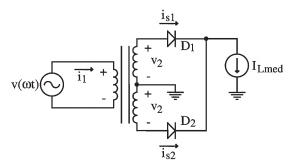
\includegraphics[scale=1.4]{imagens/estrutura_transf_onda_completa.PNG}
\caption{Circuito para o estudo do comportamento do transformador.}\label{fig:ESTOC}
\caption*{Fonte: Eletrônica de Potência (2006)}
\end{figure}

A corrente eficaz de um dos enrolamentos no secundário do transformador é
\begin{align*}
I_{sl,ef} = I_{s2l,ef} = \sqrt{ \frac{1}{2\pi}{\int_{0}^{\pi}}I_{L,med}^2{d(\omega{t})}} \\
I_{sl,ef} = I_{s2l,ef} \approx 0,707 I_{L,med} 
.\end{align*}


A potência aparente dissipada em um enrolamento do secundário é dada pela expressão \[
S_{s1} = V_{2,ef}I_{sl,ef}
.\] Como $V_{2ef} = \frac{V_{L,med}}{0,9}$, temos \[
S_{s1} \approx \frac{0,707 V_{L,med}I_{L,med}}{0,9} \approx 0,785 \,V_{L,med}I_{L,med}
.\] 

A potência aparente total no enrolamento secundário do transformador é \[
 S_{2} = S_{s1} + S_{s2}
,\] onde $S_{2} = 1,57 V_{L,med}I_{L,med}$
 Como a potência transferida à carga $P_{L} = V_{L,med}I_{L,med}$, \[
S_{2}= 1,57 P_{L}
.\] 

A tensão e a corrente no transformador se comportam conforme ilustrado na figura \ref{fig:FOC}.

\begin{figure}[ht]
\center
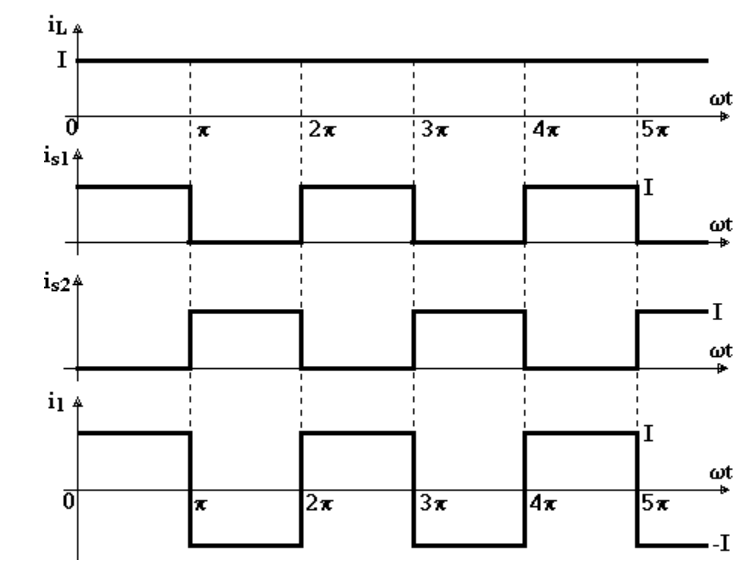
\includegraphics[scale=0.7]{imagens/FormaOndaCorrente.PNG}
\caption{Forma de onda das correntes.}\label{fig:FOC}
\caption*{Fonte: Eletrônica de Potência (2006)}
\end{figure}

Em relação ao retificador de meia onda, o retificador de onda completa se torna mais vantajoso por não resultar em uma corrente contínua no secundário do transformador, evitando a sua saturação. Além disso, a tensão média é duas vezes maior, além de resultar em uma corrente de carga com menor distorção harmônica.

